\chapter{Background}\label{chap:background}
This chapter will be divided into two subsections. The first subsection will contain definitions of terms related to citation recommendation. The second subsection explains concepts related to the algorithms used in Chapter 5.

\section{Definitions related to citations and citation recommendation}

\textbf{Citation}: \\
In the context of scientific papers, a citation is a symbolic link from a paper to papers or other external sources it references.

\textbf{Citation context}:\\
A citation context is a set of sentences which contain a reference to an external paper. Citation contexts usually have one or more citation markers, which are defined next.

\textbf{Citation marker/placeholder}: \\
A citation marker is an indicator of the location in the text where a paper has to be cited. Authors uses citation markers to point their readers to other papers which they can read for related information.
Citation markers can be of different forms. They can include the author name and year -- (Smith 2008, p. 1), or the authors and the year -- Padgett and Powell (2012), or just the reference number -- [x].

\textbf{Citing document/paper}:\\
Papers that have citation markers which point to external papers/resources are called citing papers. They contain citation markers which have corresponding entries in the reference section. The reference section contains details about the external papers/resources.

\textbf{Cited document/paper}:\\
Papers which are referenced by other (citing) papers are called cited papers. Citing papers are linked to cited papers through citation contexts and citation markers. Details about cited papers are present in the reference section of the citing paper.

Figure~\ref{fig:citingcitedpaper} shows a citing paper with a few citation contexts. Each of the citation markers in the paper, which are referenced in the reference section, point to external cited papers. 

\begin{figure}
 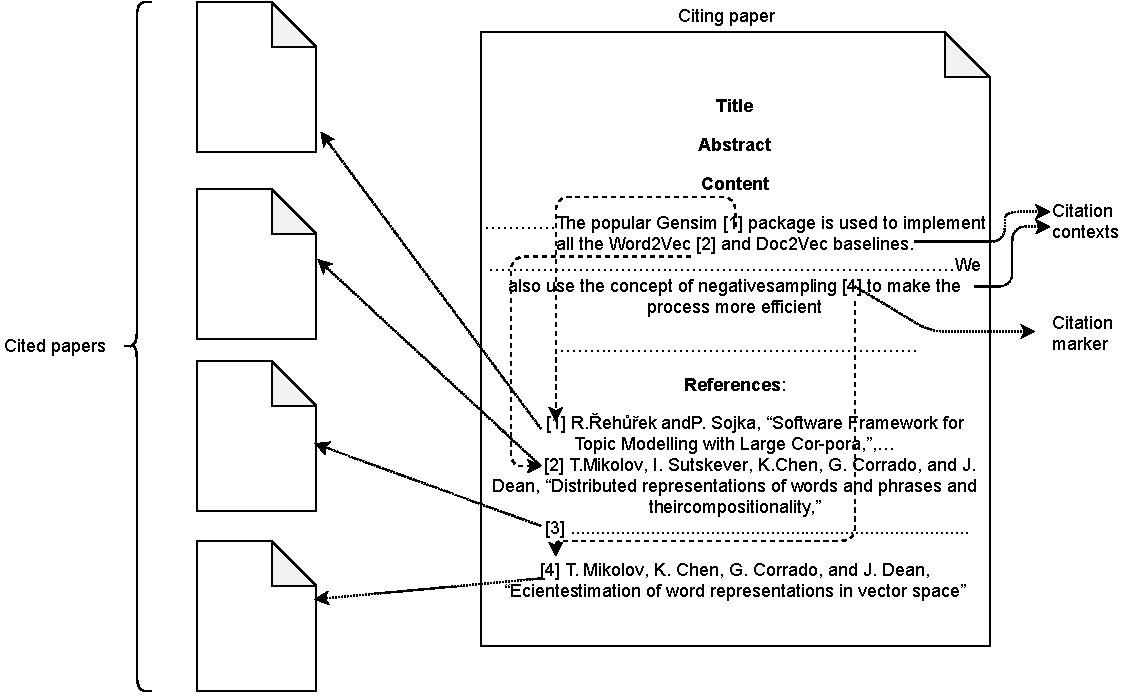
\includegraphics[keepaspectratio, width=13cm]{figures/Background/citedcitingpaper.pdf}
  \caption{Concepts related to citations}
  \label{fig:citingcitedpaper}
\end{figure}

\textbf{Citation Graph}
Citations provide a mechanism by which a set of papers can be visualised in the form of a graph G = <V,E>. Here, the Vertices V are the scientific papers themselves, which contain different citation contexts. There is an edge between two papers if one cites the other. 
A small portion of an example citation graph is shown in Figure~\ref{fig:citationgraph}. In the portion of the graph we're looking at, there are 6 papers published at different points of time. Citation markers (which are part of citation contexts) are shown in square brackets in the figure. A dashed arrow indicates that the paper at the head of the arrow is cited by the paper at the tail of the arrow. So, Paper D cites A,B and C, Paper C cites A and B, Paper E cites A and D, Paper F cites D.

\begin{figure}
 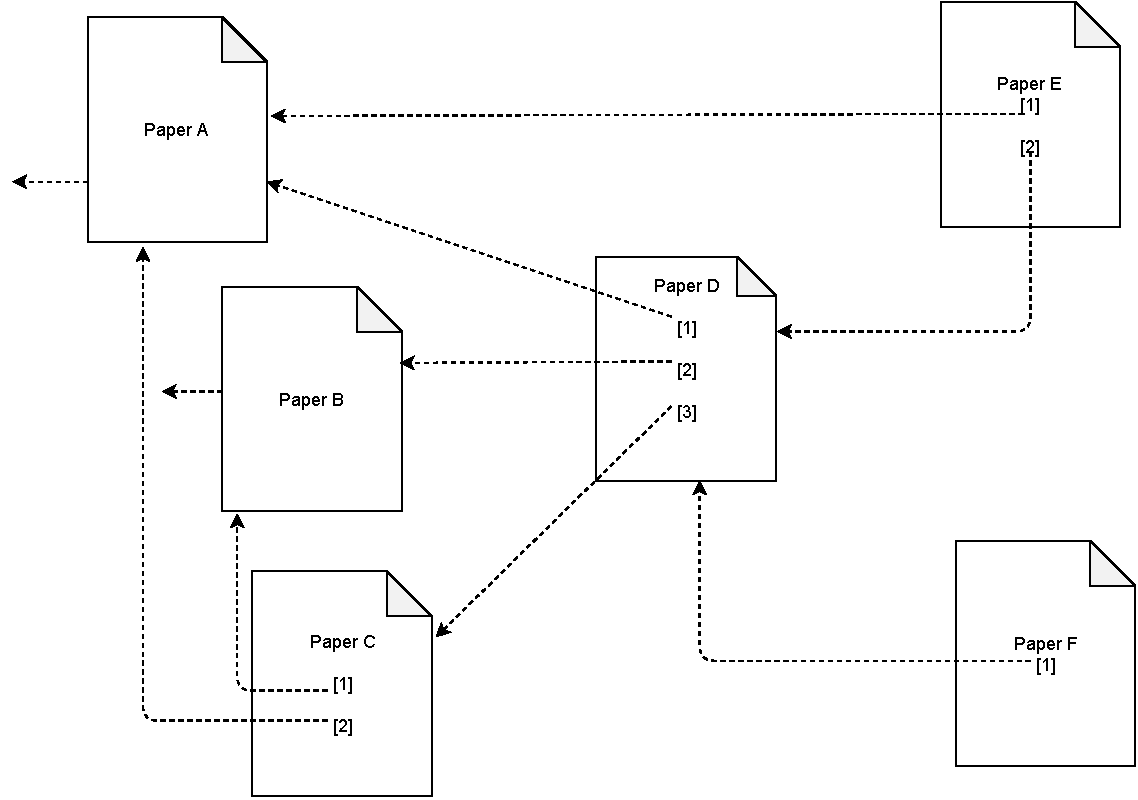
\includegraphics[keepaspectratio, width=13cm]{figures/Background/citationgraph.pdf}
  \caption{Simplified citation graph}
  \label{fig:citationgraph}
\end{figure}
\textbf{Recommender system}: \\
Recommender systems are systems which have the capability of predicting future ratings of items and recommending the predicted items with highest ratings to their users. They are in general either content-based or collaborative filtering-based.
Recommender systems are omnipresent today -- they are used in web searches, e-commerce, paper recommendation, and in a variety of other places. 

\textbf{Citation Recommendation}:\\
Citation recommendation is the process by which cited papers are recommended for citing papers. Citation recommendation can be \textit{global} or \textit{local}. 

In global citation recommendation, references in the reference section are recommended based on the entire content and/or metadata of a paper. 

Local citation recommendation, on the other hand, is the type of citation recommendation in which cited papers are recommended for a citation context. Local citation recommendation can sometimes use metadata along with the citation context as well.

E.g.: Consider the citation context, "The popular Gensim package is used to implement all the Word2Vec and Doc2Vec baselines.". The following recommendations may be retrieved for this context: \textit{Distributed Representations of Words and Phrases
and their Compositionality}\cite{MikolovSCCD13} and \textit{Software Framework for Topic Modelling with Large Corpora}\cite{rehureklrec}.

\textbf{Citation Recommendation System}:\\
This is the actual system used to carry out citation recommendation. If it is a local citation recommendation system, the user of the \textit{citation recommendation system} is recommended a particular number of papers (say, 10) for each citation context.

\textbf{Hybrid Recommender Systems}:\\
Hybrid recommender systems are recommender systems which combine the recommendations of two or more recommenders to return a single set of recommendations.
The combination can be done in a variety of ways: weighted, switching, mixed, feature combination, cascade, feature augmentation and meta-level. These are covered in detail in Burke~\cite{Burke2002}.

\textbf{Weighted hybrid recommender systems}:\\
In a weighted hybrid recommender system, the final scores for an item are computed from the corresponding scores of its composite recommender systems. A weight is assigned to each recommender system to indicate how important it is to the final recommendation. These systems make an important assumption -- \textit{that the relative value of the different techniques is more or less uniform across the space of possible items (entities to recommend)} \cite{Burke2002}. If this assumption is not satisfied, a switching or mixed system might be preferable.
Weighted hybrid recommender systems may use a linear combination of recommender scores, or can use a more complex consensus scheme.


\section{Technical concepts relating to the algorithms}

\textbf{Vector Space Model}\\
The Vector Space Model (VSM) is an important model in the field of natural language processing. In this model, words are converted into vectors. There are different models which are based on the VSM (including word embeddings), but they all follow one basic tenet: words which often occur in the same context are semenatically similar. These words are close to each other in vector space in any vector space model.

\textbf{Bag-of-words Model}\\
A bag-of-words (BOW) model is a common, but simple representation used in information retrieval. Here, a document is represented as a multiset of words. These models do not take the word order into account, but do consider the word frequency of repeated words. So, 'the man has a dog' and 'the dog has a man' will have the same BOW representations.

\textbf{Embeddings}\\
Embeddings are low-dimensional representations of high-dimensional vectors. Embeddings simplify the process of doing machine/deep learning on large inputs. A well-trained embedding places semantically similar inputs close together in the embedding space. Once an embedding is learned, it can be reused across different models.

\textbf{Word embeddings}\\
Word embeddings are embedding models which map words or phrases into numerical vectors. These vectors can be generated by different methods such as neural networks and probabilistic models. 
Word embeddings have become increasingly important in the field of natural language processing. Some popular deep-learning based word embedding models include Word2Vec \cite{MikolovSCCD13}, GloVe \cite{pennington2014glove}, FastText \cite{BojanowskiGJM16} and ELMo \cite{Peters:2018}. 

\textbf{Cosine Similarity}\\
Cosine similarity is a similarity measure used to measure the angle between two non-null vectors. It is very commonly used to compare two word vectors produced by embedding models. The smaller the angle between two word representations, the closer they are semantically. 

\textbf{Softmax}\\
In a multi-class algorithm (which is one lens through which we can look at citation recommendation), a softmax function returns probabilities for each output class.

\textbf{Word2vec}\\
Word2Vec \cite{MikolovSCCD13} is an efficient neural network-based model to compute vector representations for words. John Rupert Firth, the great English linguist, famously said, \textit{"You shall know a word by the company it keeps"}. This is the principle by which Word2Vec works. Words are predicted based on their surrounding words. 

As a result, it can be used to find synonyms and words with the same semantic relations. The stereotypical Word2Vec example shows the 'gender' semantic relation. This oft-repeated example is King: Queen, Man:?. 
Word2Vec throws up 'Woman' as the vector having the closest relation (angle) to 'Man' as 'Queen' has to 'King'. This happens because they are used in similar contexts. 

The neural network model that Word2Vec uses has an input layer, a single hidden layer and a softmax classifier as the output layer. 
The trick used in Word2Vec is that the weights of the trained neural network can be used for other tasks. Here, the size of the hidden layer is the size of each word vector. Each of the rows of the hidden layer's input weight matrix corresponds to individual word vectors. In this thesis, these word vectors will be referred to as IN word vectors. OUT word vectors come from the weights matrix between the hidden and output layers. 

OUT vectors are not generally used, but Nalisnick et al.~(\cite{NalisnickMCC16}) posit that comparing two IN vectors (IN-IN), two OUT vectors (OUT-OUT) or an IN and an OUT vector (IN-OUT) have different meanings semantically.

\textbf{Word2Vec: CBOW and Skip-Gram}\\
Word2Vec has two different flavours: Continuous Bag of Words (CBOW) and Skip-Gram. In CBOW, the target word is predicted from the surrounding source words. The window size for the number of surrounding words has to be defined. For example, consider the following sentence: 'Xi is the President of China' and a window size of 5. Here, each word is predicted in turn based on the surrounding words. After 'Xi' is predicted from  ('is', 'the', 'President', 'of', 'China'), the window slides, and the next word is predicted from its neighbours.

The Skip-gram model flips things around. Here, the surrounding words are predicted from the 'centre' word, i.e. the neighbours are predicted based on a single word. Using the same sentence as an example, the word 'China' would \textit{predict the words ('Xi', 'is', 'the', 'President', 'of'}.

For both the models, the surrounding words form a \textbf{context window} and the number of surrounding words is a hyperparameter which has to be defined.
Another important hyperparameter is the acual size of the word vectors.

\textbf{Paragraph vectors (Doc2Vec)}\\
Mikolov and Le's extension of their Word2Vec paper \cite{MikolovSCCD13} resulted in the concept of paragraph vectors \cite{LeM14}. This has been popularised as 'Doc2Vec' by the Gensim package \cite{rehureklrec}. A paragraph vector is a vector which represents the meaning of a paragraph or a whole document. 

Just like Word2Vec, Doc2Vec is trained using a similar neural network with a single hidden layer. In this thesis, we refer to the vectors from the weight matrix betweeen the input and hidden layers as the IN document vectors. The vectors from the weight matrix between the hidden and output layers are called the OUT document vectors.

\textbf{Doc2Vec PV-DM and PV-DBOW}\\
The PV-DM (Distributed memory version of paragraph vectors) is an extension of the CBOW model. Here, word vectors in the context are combined (averaged/concatenated) with a special paragraph ID to predict the centre word. 

The PV-DBOW (Paragraph Vector- Distributed Bag of Words) model is an extension of the Skip-gram model. Here, an individual document vector is used to predict the words in the document. 

Like Word2Vec, the size of the context window and the vector size are important hyperparameters. 

\textbf{Sampling rate}\\
The sampling rate is an important hyperparameter for Word2vec and Doc2Vvc which indicates the probability with which a word is kept in the vocabulary. Higher sampling rates result in many frequent words being removed from the vocabulary. 

\textbf{Negative sampling}\\
Negative sampling \cite{MikolovNegsamp} is a method used to make the training of Word2vec and Doc2vec models more efficient. While training the neural networks, only certain weights of the output layer are updated for each training example. Some negative samples are chosen for each word (words which do not often occur together are negative samples). The weights for these negative words (say, 5) and the positive word are the only weights updated, and the rest of the weights are not touched.

\textbf{Topic Modelling}\\
Topic modelling is used to discover abstract topics that occur in a collection of documents. It assigns topics to each document, such that similar documents will have a number of common topics.

\textbf{Latent Dirichlet Allocation}\\
The Latent Dirichlet Allocation (LDA) \cite{BleiNJ03} is a popular topic modelling technique which we will use as a baseline in this paper. In LDA, a document is described by a distribution of topics and a topic is described by a distribution of words. 

\textbf{Hyper-document}\\
In Han et al (\cite{ShiSZZH18}, the authors define what they call a hyper-document. A hyper-document is a collection of words and document IDs, with the document IDs substituting for citation placeholders. Consider a citing document $d_s$, which cites a document $d_t$. Let the words in the citation context be C. Then the document $d_s$ is a hyper-document which has a hyperlink <$d_s, C, d_t$>.

\textbf{Random walk}\\
A random walk in a graph is a succession of random steps in the graph. This stochastic process results in a random path being described, as well as a random destination node being reached.

\textbf{DeepWalk}\\
DeepWalk is a popular algorithm for learning node embeddings introduced by Perozzi et al (\cite{PerozziAS14}). They treat nodes as pseudo-words, and the training process is hence similar to training word embeddings. They first perform random walks on nodes in the graph. The resulting node sequences are run through the Skipgram algorithm (also used in word2vec) to get the final embeddings.

\textbf{Genetic algorithms}\\
In general, genetic algorithms are "stochastic search and optimization algorithms that mimic natural selection to find a good solution" \cite{Mueller17}. These algorithms use analogies from microbiology -- the terms to draw from are called chromosome pools. 
Genetic algorithms cover a succession of steps, as explained in \cite{Mueller17}:\\
1. Initialize Population: A random population of chromosomes is created from the chromosome pool.\\
2. Fitness score: the 'fitness' of each chromosome is evaluated using a function.\\
3. Selection: A random selection with replacement is made from the population of chromosomes based on the fitness score.\\
4. Cross-over: Pairs of chromosomes are mated -- parts of their chromosome information are exchanged.\\
5. Mutation: A low probability that some of the chromosomes may be altered or replaced is introduced.\\
6. Solution Set: Once the stopping condition is reached (when a certain fitness score is reached/a particular number of iterations is reached), the chromosomes that are left form the solution set.